\documentclass[10pt]{article}
\usepackage{graphicx}
\usepackage{amssymb}
\usepackage[fleqn]{amsmath}
\usepackage{nccmath}
\usepackage{cases}
\usepackage{hyperref}
\usepackage{pgfplots}
\usepackage{enumitem}
\pgfplotsset{compat=1.18}
\usepackage{float}
\usepackage{pdfpages}
\DeclareMathOperator*{\argmax}{argmax\,}
\DeclareMathOperator*{\argmin}{argmin\,}

\title{\bf Math 156: Problem Set 4}
\author{\bf Owen Jones}
\begin{document}
\section*{Problem 1}
\begin{align*}
    &\frac{\partial E}{\partial a_k}=-\sum_{n=1}^{N}\sum_{j=1}^{K}t_{nj}\frac{1}{y_j(\mathbf{x_n},\mathbf{w})}\frac{\partial y_j(\mathbf{x_n},\mathbf{w})}{\partial a_k}\text{ where }y_j=\frac{e^{a_j}}{\sum_{i=1}^{K}e^{a_i}}\\
    &(j=k)\frac{\partial y_j(\mathbf{x_n},\mathbf{w})}{\partial a_k}=\frac{e^{a_k}\sum_{i=1}^{K}e^{a_i}-e^{a_k}e^{a_k}}{{[\sum_{i=1}^{K}e^{a_i}]}^2}=y_k(1-y_k)\\
    &(j\neq k) \frac{\partial y_j(\mathbf{x_n},\mathbf{w})}{\partial a_k}=-\frac{e^{a_k}e^{a_j}}{{[\sum_{i=1}^{K}e^{a_i}]}^2}=-y_k y_j\\
    &\text{let }\delta_{jk}=\begin{cases}
        1 & \text{if }j=k\\
        0 & \text{otherwise}
    \end{cases}\\
    &\Rightarrow \frac{\partial E}{\partial a_k}=-\sum_{n=1}^{N}\sum_{j=1}^{K}t_{nk}\frac{1}{y_j}y_j(\delta_{jk}-y_k)\\
    &=\sum_{n=1}^{N}\sum_{j=1}^{K}t_{nj}(y_k-\delta_{jk})\\
    &\sum_{j=1}^{K}t_{nj}=1\Rightarrow\sum_{j=1}^{K}t_{nj}y_k=y_k\quad t_{n}\text{ is a one-of-K coding scheme.}\\
    &\sum_{j=1}^{K}t_{nj}\delta_{jk}=t_{nk}\delta_{kk}=t_{nk}\quad \delta_{jk}=1\text{ if }j=k\text{ and }\delta_{jk}=0\text{ otherwise.}\\
    &\text{ Thus, }\frac{\partial E}{\partial a_k}=\sum_{n=1}^{N}y_k-t_{nk}
\end{align*}
\section*{Problem 2}
Designed a neural net that contained $10$ units in its hidden layer, used a batch size of $10$, a learning rate of $0.001$, a tolerance of $0.1$, and $1000$ as the maximum number of iterations. 
Obtained a $99.5\%$ accuracy on training data and $110\%$ accuracy on the test data.
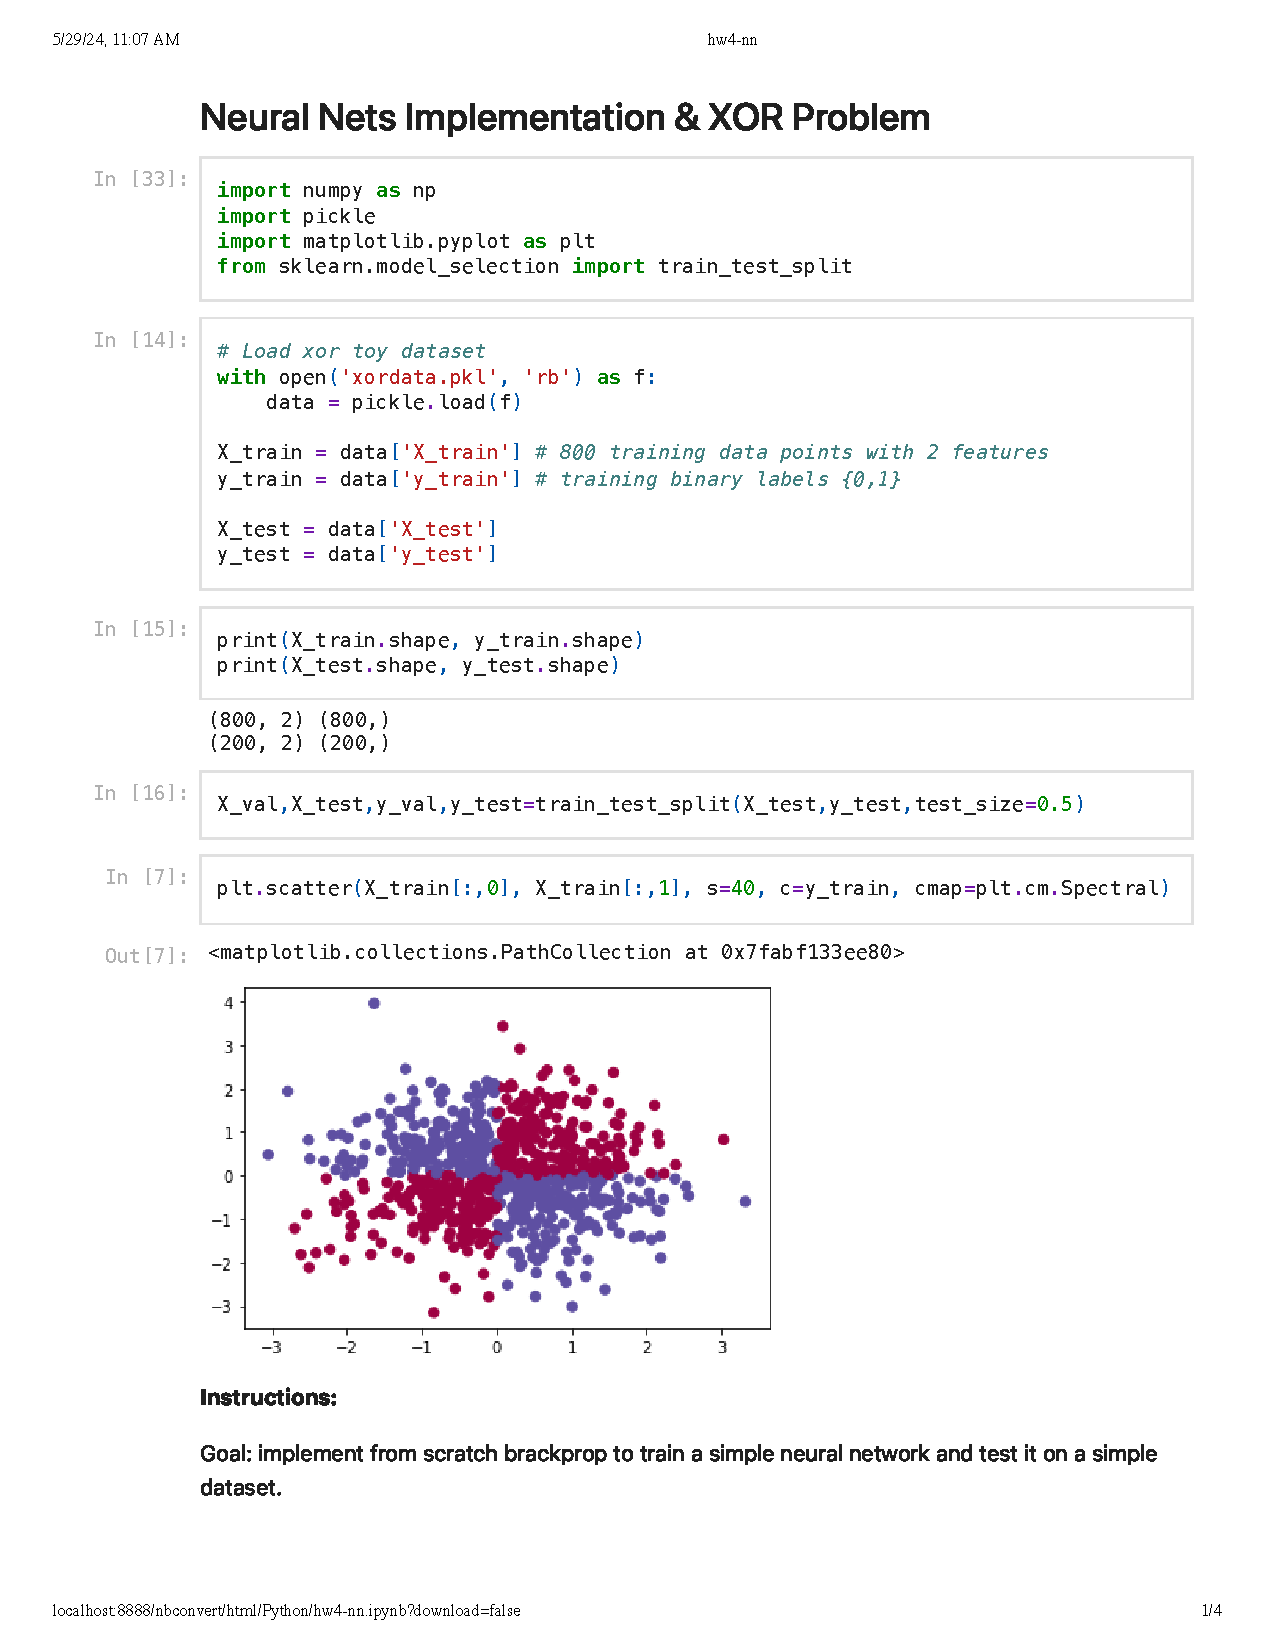
\includepdf[pages=-]{hw4-nn.pdf}
\end{document}